\subsection{稳态转换潜在驱动期分析}

首先,本章研究检测到的驱动力时段(两个气候驱动和两个人类活动驱动)均能够在既有研究中得到印证。
(1)从900年到公元$1100$年的CDP1是一个典型的潮湿时期,通常被称为“中世纪暖期”\cite{zhang1993, zhang1994, man2014},此时期温暖而潮湿的气候让通常会引发农业范围的北扩\cite{TanQiXiang1996,GeQuanSheng2011}。
(2)第二个气候驱动期(公元$1700$年到$1900$年,CDP2)几乎覆盖了整个中国古代清朝,包括此时开始的我国最早的系统性气象观测资料——“雨雪分寸”在内的各种数据反演结果都能表明,这是一个典型的湿期\cite{hao2021, ge2008}。
(3)本章研究识别的第一个人类活动驱动时期持续时间较长(公元$1350$年至公元$1650$年,HDP1),而根据 Wang 等人的考证,这段时间靠中间的公元1491年,黄土高原人口迅速增加到$1150$万,且有着土地复垦加速的可信记录\cite{wang2006b}。
(4)第二个人类活动驱动时期(1900以后,HDP2)已是近代,史料较为丰富切翔实可靠,期间除了快速增长的人口也记录了频繁的土地纠纷,以及黄河中游强烈的开垦和农业土地利用\cite{GeJianXiong2005}。
其次,影响因素的组合作为识别稳态转换过程的潜在参考,能展示更多关于变化时期的信息,同样也得到了前人研究的佐证。
在潮湿的气候驱动期,增加的降水同时提升了洪泛频次、土壤侵蚀、与泥沙沉积\cite{chen2012}。
此外,此时期的湿润气候也有利于三门峡谷通行,而这正是北宋政府沿着黄河水路运输的粮食的关键\cite{WangShouChun1993}。

\subsection{稳态转换的发生过程与机制}

本章研究可以在历史时期对黄河如何进入受人类活动主导的稳态做如下解释。
首先,在潮湿的第一个气候驱动时期中发生的变化(即沉积速率增加,更频繁的洪泛,以及航运得到改善)在此时期后,仅沉积速率保持相对不变(可能源于有限的农业扩张,但数据可信度较弱),而航运情况与洪泛情况都重新回到此时期前的水平。
因此,尽管潮湿的气候与人类活动都有所体现,但此时期仍然是气候变化为主要驱动力,且稳态转换的临界点尚未到来(图\ref{fig:ch3:regime_shift}~A)。
接下来的人类活动驱动时期(HDP)期间,持续增强的开垦压力导致影响因素的组合产生了一些差异(见图\ref{fig:ch3:impacts}~从C到D),因此在CDP2期间,潮湿的气候仅影响洪水的频率而未能缓解三门峡通航的困难。
最后,在第二个气候驱动期(CDP2)也结束之后迎来了新的人类活动驱动期(HDP2),仅有洪泛频率退回到潮湿期之前的水平,而泥沙沉积速率仍在增加,通航状况也陷入了历史最糟糕的时期。所有这些迹象表明稳态转换已经发生,人类活动已经主导了黄河流域,自1350年以来不断增加的人为压力已将稳态推出了气候周期规律(图\ref{fig:ch3:regime_shift}~B)。

\begin{figure}[!h] % use float package if you want it here
    \centering{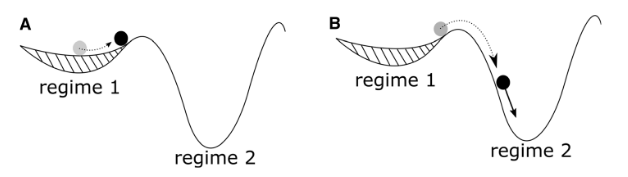
\includegraphics[width=0.8\textwidth]{img/ch3/ch3_regime_shift.png}}
    \caption[历史时期黄河流域水沙特征由人类活动主导的过程]{黄河流域转向人类活动主导的稳态转换过程解释图。稳态1和稳态2分别表示原始状态下自然驱动力主导的黄河与人类活动主导的黄河。灰色的圆圈用虚线箭头表示流域系统在气候驱动力下的状态。黑色圆实心箭头表示不断增强的人为压力。A图所示的变化反映了从公元$400$年到公元$1350$年的过程(对应于图\ref{fig:ch3:impacts}的从A到C)。B图所示的变化为从1350年到公元2000年(对应于图\ref{fig:ch3:impacts}的从D到F)。}\label{fig:ch3:regime_shift}
\end{figure}
